\documentclass{beamer}

\usepackage{polski}
\usepackage[utf8]{inputenc}
\usepackage{graphicx}
\usepackage{listings}
\usepackage{adjustbox}
\usepackage{verbatim} 
\usepackage{color}

\definecolor{gray}{rgb}{0.4,0.4,0.4}
\definecolor{darkblue}{rgb}{0.0,0.0,0.6}
\definecolor{cyan}{rgb}{0.0,0.6,0.6}
\usepackage{relsize}

%c C sharp
\def\Csharp{%
    C\kern-.1667em\raise.30ex\hbox{\smaller{\#}}%
 }

\title{Proces wytwarzania oprogramowania na platformę Windows Runtime na przykładzie aplikacji biznesowej.}   
\subtitle{Pracownia dyplomowa I}
\author{Paweł Sołtysiak} 
\institute{Opiekun pracy: dr inż.  Witold Maćków\\Kierownik Katedry: prof. dr hab. inż. Włodzimierz Bielecki}
\date{\today} 


\begin{document}


\begin{frame}
\titlepage
\end{frame} 

\begin{frame}
\frametitle{Agenda} 
\tableofcontents
\end{frame} 

\begin{frame}
\section{Cel pracy}
\frametitle{Cel pracy -- Cześć teoretyczna} 
Przedstawienie metodyki wytwarzania oprogramowania dla platformy Windows Runtime na przykładzie aplikacji biznesowej.
\end{frame}

\begin{frame}
\frametitle{Cel pracy -- Cześć praktyczna} 
Projekt i implementacja aplikacji w oparciu o wybrane metodologie, wzorce i technologie.
\end{frame}

\begin{frame}
\frametitle{Zakres pracy} 
\section{Zakres pracy}
Opis architektury Windows 8 Runtime. Przegląd metodologii, wzorców i technologii dedykowanych do wytwarzania oprogramowania dla przedstawionej architektury. Określenie i analiza wymagań projektowych aplikacji.\\
~\\
Projekt i implementacja aplikacji w oparciu o wybrane metodologie, wzorce i technologie. Testy opracowanej aplikacji. Określenie stosowalności przedstawionego procesu wytwarzania oprogramowania dla szerszej klasy aplikacji.
\end{frame}


\begin{frame}
\frametitle{Uzasadnienie wyboru pracy} 
\begin{itemize}
\item Praca zawodowa dotycząca Windows 8 i programowania w Windows Runtime.
\item Poszerzenie i pogłębienie wiedzy na temat Windows Runtime.
\item Tematyka związana z inżynierią oprogramowania
\item Przyszłość należy do urządzeń mobilnych 
\end{itemize}
\end{frame}


\begin{frame}
\section{Zadania pracy}
\frametitle{Zadania pracy w części teoretycznej}
\begin{itemize}
\item Opis architektury Windows Runtime.
\item Przegląd metodologii, wzorców i technologii dedykowanych do wytwarzania oprogramowania dla przedstawionej architektury.
\item Określenie i analiza wymagań projektowych aplikacji.
\item Określenie stosowalności przedstawionego procesu wytwarzania oprogramowania dla szerszej klasy aplikacji.
\end{itemize} 
\end{frame}


\begin{frame}
\frametitle{Zadania pracy w części praktycznej}
\begin{itemize}
\item  Projekt i implementacja aplikacji w oparciu o wybrane metodologie, wzorce i technologie.
\item Testy opracowanej aplikacji. 
\end{itemize}
\end{frame}


\section{Spis treści}
\begin{frame}
\frametitle{Spis treści}
\begin{enumerate}
\item Wstęp
\begin{enumerate}
\item Wprowadzenie
\item Cel pracy
\item Struktura pracy
\end{enumerate}

\item Cześć teoretyczna

\begin{enumerate}

\item Środowisko
\begin{enumerate}
\item Windows 8
\item Windows Runtime

\end{enumerate}


\item Narzędzia i Technologie
\begin{enumerate}
\item Visual Studio 2012

\item Dostępne języki programowania
\begin{enumerate}
\item C\#
\item C++
\item JavaScript
\end{enumerate}

\item Języki opisu interfejsu użytkownika
\begin{enumerate}
\item XAML
\item HTML
\end{enumerate}
\item Baza danych SQLite
\end{enumerate}

\item Zadania  aplikacji biznesowej
\end{enumerate}
\end{enumerate}

\end{frame}

\begin{frame}
\frametitle{Spis treści}

\begin{enumerate}
\setcounter{enumi}{2}
\item Cześć praktyczna
\begin{enumerate}
\item Analiza wymagań

\item Model danych

\item Schematy funkcjonowania aplikacji
\begin{enumerate}
\item Diagram przypadków użycia
\item Diagram przepływu danych
\end{enumerate}

\item Tworzenie interfejsu użytkownika
\begin{enumerate}
\item Wykorzystanie Model View View-Model
\item Tworzenie interfejsu dotykowego
\end{enumerate}

\item Wykorzystanie SQLite

\end{enumerate}
\item Implementacja i testy
\item Przykład działania aplikacji
\item Podsumowanie
\item Bibliografia

\end{enumerate}


\end{frame}



\begin{frame}
\begin{itemize}
\frametitle{Metoda badawcza}
\item Metoda intuicyjna - obecna w każdej metodzie badań naukowych. 
\item Metoda obserwacyjna
\end{itemize}
\end{frame}

\section{Część teoretyczna}
\begin{frame}
\frametitle{Zawartość części teoretycznej}
Opis użytych narzędzi podczas budowania aplikacji biznesowej razem z uzasadnieniem.
Między innymi:
\begin{itemize}
\item Zadania aplikacji biznesowej
\item Windows 8 i Platforma Windows Runtime
\item Visual Studio
\item Języki programowania
\item Języki opisu interfejsu użytkownika
\item Baza danych SQLite
\end{itemize}
\end{frame}


\begin{frame}
\frametitle{Zadania aplikacji biznesowej}
Przykładowe zadania aplikacji biznesowej
\begin{itemize}
\item	Bezpieczny dostęp do danych w firmie
\item	Przeglądanie danych pochodzących z firmy
\item	Umieszczanie danych
\end{itemize}
\end{frame}

\begin{frame}
\frametitle{Windows 8}
Windows 8 jest wersją systemu operacyjnego Microsoft Windows, produkowanego przez Microsoft przeznaczoną do użytku na komputerach osobistych, włączając w to domowe i firmowe komputery stacjonarne, laptopy i tablety PC.
\end{frame}

\begin{frame}
\frametitle{Windows Runtime}
Windows Runtime lub w skrócie WinRT jest jednolitą platformą do tworzenia aplikacji w systemie operacyjnym Windows 8. Windows Runtime pozwala na natywne programowanie w języku C++/CX oraz na programowanie przy użyciu języków zarządzalnych takich jak \Csharp i \texttt{VB.NET}, a także \texttt{JavaScript}. Dzięki platformie Windows Runtime programy mogą być natywnie uruchamiane na procesorach x86 oraz ARM w trybie piaskownicy.
\end{frame}

\begin{frame}
\frametitle{Windows Runtime -- biblioteka}
Windows Runtime jest oparte na COM (Component Object Model). Wykorzystanie COM pozwala na utworzenie wspólnego interfejsu programistycznego z wszystkimi językami programowania.
\end{frame}

\begin{frame}
\frametitle{Visual Studio}
\begin{itemize}
\item	Wymagana licencja deweloperska
\item	Przykładowy kod aplikacji
\item	Wizualny edytor interfejsu użytkownika
\item	Edytor kodu
\item	Dystrybucja -- deployment
\item	Lokalizacja
\item 	Debugowanie i testowanie (testy jednostkowe)
\end{itemize}
\end{frame}

\begin{frame}
\frametitle{Języki programowania}
\begin{itemize}
\item	JavaScript
\item	\Csharp
\item	\texttt{C++/CX}

\end{itemize}
\end{frame}

\begin{frame}
\frametitle{Języki opisu interfejsu użytkownika}
\begin{itemize}
\item	XAML
\item	HTML
\end{itemize}
\end{frame}

\lstset{
  basicstyle=\ttfamily,
  columns=fullflexible,
  showstringspaces=false,
  commentstyle=\color{gray}\upshape
}

\lstdefinelanguage{XML}
{
  morestring=[b]",
  morestring=[s]{>}{<},
  morecomment=[s]{<?}{?>},
  stringstyle=\color{black},
  identifierstyle=\color{darkblue},
  keywordstyle=\color{cyan},
  morekeywords={xmlns,version,type}% list your attributes here
}

\begin{frame}[fragile]
\frametitle{XAML}
 \begin{adjustbox}{width=\textwidth}
\begin{lstlisting}[language=XML,basicstyle=\ttfamily]

<Grid x:Name="LayoutRoot" Background="White" 
      HorizontalAlignment="Left" VerticalAlignment="Top"> 
        <Grid.RowDefinitions> 
            <RowDefinition Height="Auto"/> 
            <RowDefinition Height="*"/> 
        </Grid.RowDefinitions> 
        <Grid x:Name="Input" Grid.Row="0"> 
            <Grid.RowDefinitions> 
                <RowDefinition Height="Auto"/> 
                <RowDefinition Height="*"/> 
            </Grid.RowDefinitions> 
            <TextBlock x:Name="Scenario1Input"  TextWrapping="Wrap" 
            Grid.Row="0" Style="{StaticResource BasicTextStyle}" HorizontalAlignment="Left" > 
                Displays the profile information for the Internet Connection Profile. 
            </TextBlock> 
            <StackPanel Orientation="Horizontal" Margin="0,10,0,0" Grid.Row="1"> 
                <Button x:Name="InternetConnectionProfileButton" 
                Content="Get Internet Connection Profile Info" 
                Margin="0,0,10,0" Click="InternetConnectionProfile_Click"/> 
            </StackPanel> 
        </Grid> 
</Grid> 
\end{lstlisting}
\end{adjustbox}
\end{frame}

\begin{frame}[fragile]
\frametitle{HTML}
 \begin{adjustbox}{width=\textwidth}
\begin{lstlisting}[language=XML,basicstyle=\ttfamily]
<html> 
<head> 
    <meta charset="utf-8" /> 
    <title>SDK Sample</title> 
    <!-- WinJS references --> 
    <link rel="stylesheet" href="//Microsoft.WinJS.1.0/css/ui-light.css" /> 
    <script src="//Microsoft.WinJS.1.0/js/base.js"></script> 
    <script src="//Microsoft.WinJS.1.0/js/ui.js"></script> 
 
    <!-- SDK sample framework references --> 
    <link rel="stylesheet" href="/sample-utils/sample-utils.css" /> 
    <link rel="stylesheet" href="/css/default.css" /> 
    <script src="/sample-utils/sample-utils.js"></script> 
    <script src="/js/default.js"></script> 
</head> 
<body role="application"> 
    <div id="rootGrid"> 
        <div id="header" role="contentinfo" data-win-control="WinJS.UI.HtmlControl" 
        data-win-options="{uri: '/sample-utils/header.html'}"></div> 
        <div id="content"> 
            <h1 id="featureLabel"></h1> 
            <div id="contentHost"></div> 
        </div> 
        <div id="footer" data-win-control="WinJS.UI.HtmlControl" 
        data-win-options="{uri: '/sample-utils/footer.html'}"></div> 
    </div> 
</body> 
</html> 
\end{lstlisting}
\end{adjustbox}
\end{frame}

\begin{frame}
\frametitle{SQLite}
SQLite – to system zarządzania bazą danych oraz biblioteka C implementująca taki system, obsługująca język SQL (ang. Structured Query Language). Została stworzona przez Richarda Hippa i jest dostępna na licencji public domain.\\
~\\
https://github.com/praeclarum/sqlite-net
\end{frame}


\section{Część praktyczna}
\begin{frame}
\frametitle{Zawartość części praktycznej}
Budowanie aplikacji, przy wykorzystaniu opisanych wcześniej narzędzi.

Poruszę takie tematy jak:
\begin{itemize}
\item Analiza wymagań
\item Diagramy przypadków użycia
\item Projekt modelu danych
\item Interfejs użytkownika
\item Implementacja programu w języku \Csharp
\item Testy jednostkowe
\end{itemize}
\end{frame}

\begin{frame}
\frametitle{Przykładowa aplikacja}
 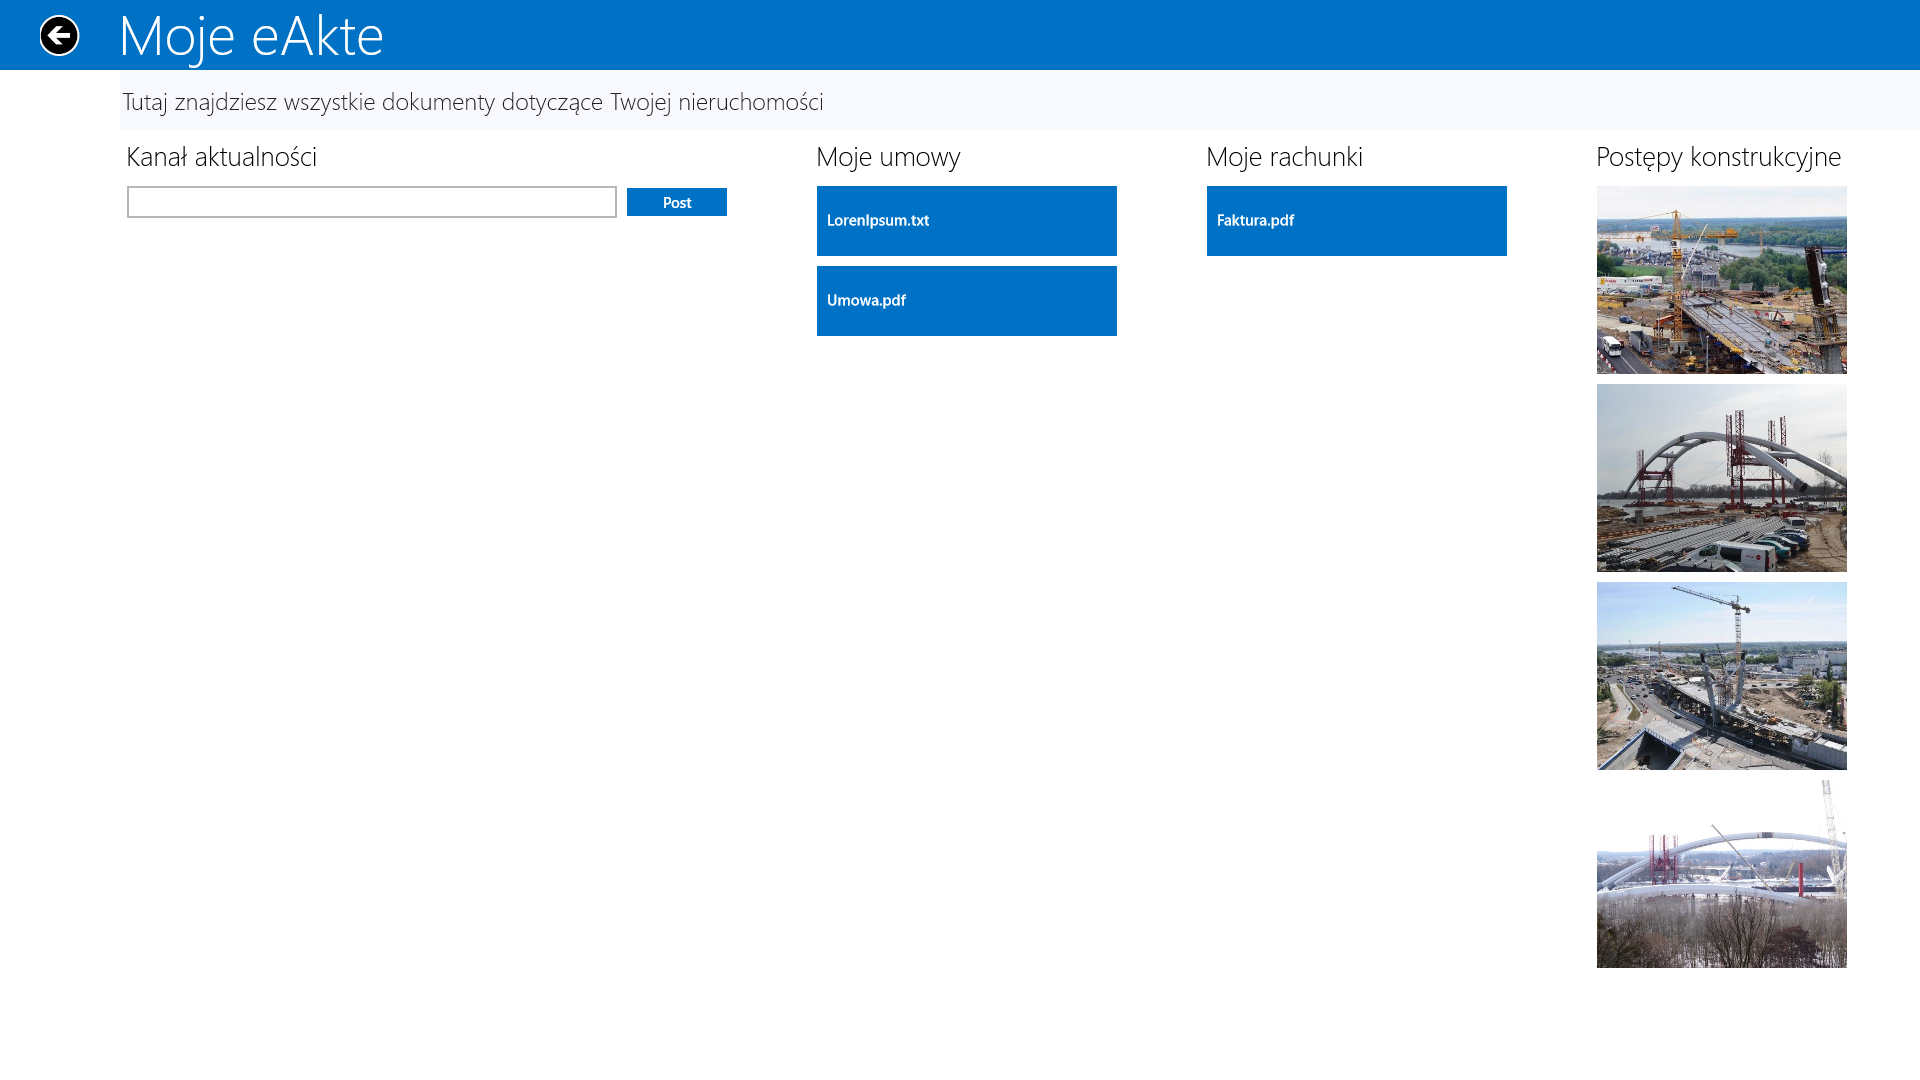
\includegraphics[width=\textwidth]{screenshot.png}
\end{frame}

\begin{frame}
\frametitle{Trudności w realizacji zadań pracy}

\begin{itemize}
\item ,,Problemy wieku młodzieńczego'' Windows 8 oraz Windows Runtime.
\item Brak ,,dojrzałych'' bibliotek dla platformy Windows Runtime.
\item Ograniczenia sprzętowe.
\item Brak czasu
\item Brak literatury
\end{itemize}
\end{frame}


\begin{frame}
\frametitle{Bibliografia} 
\begin{itemize}
\item Code Complete 
\item Patterns of Enterprise Application Architecture
\item \href{http://msdn.microsoft.com/en-us/windows/apps/}{MSDN -- Windows Store apps}
\item \href{http://www.charlespetzold.com/blog/2013/01/Programming-Windows-6th-Edition-Final-Ebook-Now-Available.html}{Programming Windows 6th Edition -- Charles Petzold}
\end{itemize}
\end{frame}


\begin{frame}
\frametitle{Harmonogram} 
\begin{itemize}

\item 02.13 – 05.13 Zapoznanie się z literaturą i technologiami
\item 06.13 – 09.13 Implementacja aplikacji, testy
\item 10.13 – 12.13 Opis części teoretycznej i praktycznej
\item 01.14 Ostatnie poprawki pracy

\end{itemize}
\end{frame}


\begin{frame}
\frametitle{Dziękuje za uwagę...}
Pytania?

\end{frame}
\end{document}
